\section{Tensat: Optimizing Deep Learning Computation Graphs}
\label{sec:tensat}

\newcommand{\ourname}{Tensat\xspace}
\newcommand{\tensat}{Tensat\xspace}

Deep learning frameworks and compilers
 (e.g., Tensorflow~\cite{TensorFlow}, PyTorch~\cite{NEURIPS2019_9015},
  XLA~\cite{xla}, TensorRT~\cite{TensorRT}, TVM~\cite{tvm},
  MLIR~\cite{mlir})
 have enabled diverse kinds of machine learning models to run
 efficiently on numerous compute platforms.
Neural network models in
 these frameworks are typically represented as tensor computation
 graphs.
To improve the runtime performance of a tensor graph, these
 frameworks perform various optimizations.

One of the most important optimizations is graph rewriting,
 which takes in a tensor graph $g$ and a set of semantics-preserving graph rewrites $R$,
 and by applying rewrites to $g$ seeks to find an semantically equivalent $g'$ with lower cost according to some cost model.
% which transforms a tensor graph by iteratively applying rewrite rules that substitute subgraphs with semantically equivalent ones.
%The graph rewriting optimization problem can be factored into two sub-problems: (1) discovering a comprehensive set of rewrite rules and (2) an algorithm that determines the order in which to apply the rewrite rules to optimize a given graph.
The current industry-standard approach adopted by most frameworks is to use a manually curated set of rewrite rules and rely on a heuristic strategy to determine the order in which to apply the rewrite rules.
%that often applies rewrite rules greedily.
However, this approach often leads to sub-optimal results both due to the non-comprehensive set of rewrite rules, as well as the sub-optimal graph substitution heuristic \cite{taso,metaflow}. % that considers only a small fraction of all possible graphs reachable with a given set of rewrites \cite{taso, metaflow, Fang:sampling}.

This case study aims to address the sub-optimality problem of graph rewrite strategies, while leveraging the existing rewrite rules generation technique~\cite{taso}.
Prior research has shown that searching for sequences of substitutions
\cite{taso,metaflow,Fang:sampling} outperforms heuristic approaches.
However, both heuristic and search-based solutions rely on sequential application of substitutions.
Since rewrites often depend on or enable one another,
optimization depends heavily on the order in which rewrites are applied;
the ``phase ordering'' problem strikes again.
% this classically tricky problem is known in the compilers community as the ``phase-ordering'' or ``rewrite-ordering'' problem.


\begin{table}[]
    \centering
    \begin{tabular}{ccc|cc}
    \hline
    & \multicolumn{2}{c|}{\bf Search time (s)} & \multicolumn{2}{c}{\bf Runtime speedup (\%)} \\
    & TASO & \ourname{} & TASO & \ourname{} \\
    \hline
    BERT & 13.6 & \textbf{1.4} & 8.5 & \textbf{9.2} \\
    ResNeXt-50 & 25.3 & \textbf{0.7} & 5.5 & \textbf{8.8} \\
    NasNet-A & 1226 & \textbf{10.6} & 1.9 & \textbf{7.3} \\
    NasRNN & 177.3 & \textbf{0.5} & 45.4 & \textbf{68.9} \\
    Inception-v3 & 68.6 & \textbf{5.1} & 6.3 & \textbf{10.0} \\
    SqueezeNet & 16.4 & \textbf{0.3} & 6.7 & \textbf{24.5} \\
    VGG-19 & 8.9 & \textbf{0.4} & \textbf{8.9} & \textbf{8.9} \\
    \hline
    \end{tabular}
    \caption{Comparison of optimization time and runtime speedup of the optimized computation graphs over the original graphs, TASO~\cite{taso} v.s. \ourname{}.}
    \label{table:ngraph}
\end{table}


This case study presents \ourname{}, a tensor graph superoptimization framework that employs equality saturation \cite{eqsat, eqsat-llvm, egg},
to apply all possible rewrites at once.  %comprehensively and scalably explore the search space of all equivalent graphs a given a set of rewrite rules.
\tensat splits program optimization into two phases: {\em exploration} and {\em extraction}.
The exploration phase is equality saturation using \egg as usual.
\tensat's extraction phase is totally custom;
 simple cost functions simply do not suffice for extracting efficient deep learning compute graphs.
Instead, \tensat employs an Integer Linear Programming (ILP) extraction solution,
 which requires
 a novel method to filter out invalid subgraphs from an e-graph.
% The extraction phase selects from the e-graph the equivalent program with the lowest cost according to a given cost model. The compact representation of the exponentially large search space using e-graphs enables extraction algorithms that can find the globally optimal equivalent program quickly.
%\ourname{} uses equality saturation to replace the heuristic- or sequential-search-based rewriting approaches from prior work.

% Applying equality saturation to tensor graph rewriting requires non-trivial extensions in both the exploration and extraction phases.
% We extend the exploration phase to support complex, non-local rewrite rules that are necessary to produce highly efficient tensor graphs.
% Additionally, we introduce a novel method to filter out invalid subgraphs from an e-graph,
% which enables our extraction procedure based on Integer Linear Programming (ILP) to quickly find the optimal solution.

We evaluated \ourname{} on a number of well-known machine learning models executing on a GPU.
As highlighted in \autoref{table:ngraph}, \ourname{} can synthesize optimized graphs that are up to 23\% faster in runtime than state-of-the-art \cite{taso}, while reducing the optimization time by up to 300x.
By having the e-graph compactly representing an exponential number of equivalent graphs, \ourname{} is able to cover a larger search space more efficiently than the sequential search methods.
As a result, our search approach is both extremely effective and fast enough to be used as part of a normal complation flow.
%Our approach discovers better optimized graphs than the state-of-the-art, at the same time running much faster such that it can be used as part of a normal compilation flow.
%We believe that our approach is the first tensor graph superoptimization that is both \ATTN{provably optimal} and fast enough to be used as part of a normal complation flow.

%However, doing so requires non-trivial extensions in both the saturation as well as the extraction phase: (a) extending equality saturation to support complex rewrite rules (b) formulating the extraction problem as a integer linear programming(ILP), and (c) designing pruning strategies to trade-off coverage (in terms of the number of graphs explored) for shorter time to solve the ILP problem.


%We evaluated \ourname{} on a number of well-known machine learning models (including BERT, ResNeXt-50, NasNet-A, NasRNN, and Inception-v3), comparing against TASO \cite{taso}, state-of-the-art tensor graph rewriting approach.
%up to xxx faster performing graphs in up to xxx smaller search time while exploring an exponentially larger search space.
%In addition, we have also performed a number of ablation studies to highlight the importance of the specific optimizations and extensions proposed in this paper.

\subsection{Representation}

This section describes how \ourname{} represents tensor computation graphs and rewrite rules.

\paragraph{Representing Tensor Computation Graphs}
\label{sec:language}

We use a representation based on the one in TASO~\cite{taso},
 with modifications to make it suitable for equality saturation.
\autoref{table:ops} shows the set of operators we consider.
Each operator $o_i$ corresponds to a node $n_i$ in the graph; the node represents the output tensor of the operator.
The nodes corresponding to the inputs of $o_i$ are the children nodes of $n_i$.
% Unlike TASO, we include both the input tensors and the operator parameters as the children nodes of the operator node.
% This way, all the relevant information of the tensor computation graph is represented syntactically by the nodes and the edges, without the need of additional annotations on the nodes.
Each tensor computation graph is a DAG under this representation.

The formulations in equality saturation become simpler if a graph is
single-rooted. Therefore, we combine all the final output nodes of a
graph with \emph{no-op}s to make the graph single-rooted. The no-op
nodes do not have any actual operators associated with them, and they
will not be altered during the exploration phase, so there are no side
effects.


\begin{table}[t]
    \centering
    \newcommand\act{\textsf{activation}}
    \newcommand\width{\textsf{w}}
    \newcommand\height{\textsf{h}}
    {\textbf{Types}
      \\[1mm]
      \small
    \begin{tabular}{cl|cl|cl|cl}
      $T$ & Tensor
      & $TT$ & Tensor tuple
      & $W$ & Weights tensor
      & $s_\height, s_\width$ & stride (height, width) \\
      $n$ & natural number
      & $p$  & padding
      & $a$ & activation
      & $k_\height, k_\width$ & kernel (height, width) \\
    \end{tabular}}
    \\[2em]
    \begin{tabular}{lll}
        {\bf Operator}  & {\bf Description}                    & {\bf Type signature} \\
    \hline
        \sf ewadd           & Element-wise addition                & $(T, T) \rightarrow T$ \\
        \sf ewmul           & Element-wise multiplication          & $(T, T) \rightarrow T$ \\
        \sf matmul          & Matrix multiplication                & $(a, T, T) \rightarrow T$ \\
        \sf conv $^a$       & Grouped convolution                  & $(s_\height, s_\width, p, a, T, W) \rightarrow T$ \\
        \sf relu            & Relu activation                      & $T \rightarrow T$ \\
        \sf tanh            & Tanh activation                      & $T \rightarrow T$ \\
        \sf sigmoid         & Sigmoid activation                   & $T \rightarrow T$ \\
        \sf poolmax         & Max pooling                          & $(T, k_\height, k_\width, s_\height, s_\width, p, a) \rightarrow T$ \\
        \sf poolavg         & Average pooling                      & $(T, k_\height, k_\width, s_\height, s_\width, p, a) \rightarrow T$ \\
        \sf transpose $^b$  & Transpose                            & $(T, {\sf permutation}) \rightarrow T$ \\
        \sf enlarge $^c$    & Pad a convolution kernel with zeros  & $(T, T_{\sf ref}) \rightarrow T$ \\
        \sf concat$_n$ & Concatenate along the given axis     & $(n, T, \dots, T) \rightarrow T$ \\
        \sf split $^d$      & Split a tensor into two along the axis & $(n, T) \rightarrow TT$ \\
        \sf split$_0$       & Get the first output from split      & $TT \rightarrow T$ \\
        \sf split$_1$       & Get the second output from split     & $TT \rightarrow T$ \\
        \sf merge $^e$      & Update weight to merge grouped conv  & $(W, n) \rightarrow W$ \\
        \sf reshape         & Reshape tensor                       & $(T, {\sf shape}) \rightarrow T$ \\
        \sf input           & Input tensor                         & ${\sf identifier} \rightarrow T$ \\
        \sf weight          & Weight tensor                        & ${\sf identifier} \rightarrow T$ \\
        \sf no-op            & Combine the outputs of the graph     & $(T, T) \rightarrow T$ \\
    \end{tabular}
    \\[1em]
    \caption{
        Operators supported by \ourname.
        There are four types for the nodes in our representation:
        tensor type (T), string type (S), integer type (N), and tensor tuple type (TT).
        The integer type is used to represent parameters of the
         operators, such as stride, axis, and also padding and activation modes
         (by representing different modes using different integers).
         The more complex, variable-length parameters
          (e.g. shape, axes permutation) are represented using the
          string type according to the specified formats.
          \\[1em]
          \footnotesize{
            $^a$ Same representation as TASO \cite{taso}.
                 Normal and depth-wise convolutions are special cases
                 of grouped convolutions. \\
            $^b$ Axis permutation for transpose is specified
                 using a string with format: axis$_1$\_axis$_2$\_\dots .\\
            $^c$ Pad a convolution kernel (input) with
                 zeros to make it the same size as input $T_{\sf ref}$ \\
            $^d$ Split the tensor in the given axis. The position of the split is at the place of the most recent concat. \\
            $^e$ Merge every \textit{count} number of groups in the grouped convolution. See TASO \cite{taso} for more details. \\
          }
    }\label{table:ops}
\end{table}


\paragraph{Representing Rewrite Rules}
\label{sec:rewrite}

A rewrite rule for tensor computation graph specifies that some local subgraph pattern (\textit{source pattern}) is equivalent to another subgraph pattern (\textit{target pattern}).
The input tensors to the source and target patterns are \textit{variable nodes}, which can be substituted with any concrete nodes (or e-class in equality saturation) in the current graph.
Each output tensor in the source pattern corresponds to an output tensor in the target pattern.
The two corresponding output nodes are called a pair of \textit{matched outputs}.
A rewrite rule states the equivalence between each pair of matched outputs.

We represent each source (and target) pattern using symbolic expressions (S-exprs) with variables.
Patterns with a single output is represented with an S-expr rooted on the output.
Rewrite rules with such patterns are called \textit{single-pattern rewrite rules}.
Patterns with multiple outputs are represented as a list of S-exprs rooted on each output.
Rewrite rules with multiple matched outputs are called \textit{multi-pattern rewrite rules}.
% \autoref{fig:rewrite} shows an example rewrite rule and its representation.

% \begin{figure}[t]
%     \centering
%     \includegraphics[width=\linewidth, draft=true]{figures/rewrite-example.pdf}
%     \begin{scriptsize}
%     Source: (matmul ?input$_1$ ?input$_2$), (matmul ?input$_1$ ?input$_3$) \\
%     Target: (split$_0$ (split 1 (matmul ?input$_1$ (concat$_2$ 1 ?input$_2$ ?input$_3$)))), \\
%     (split$_1$ (split 1 (matmul ?input$_1$ (concat$_2$ 1 ?input$_2$ ?input$_3$))))
%     \end{scriptsize}
%     \caption{
%     Example rewrite rule and its representation in S-expressions.
%     Identifiers starting with "?" denote variable nodes.
%     For clarity, we omit the activation mode inputs to \texttt{matmul}.
%     Arrows point from parent nodes to children nodes.
%     1 is the axis for \texttt{split} and \texttt{concat} operators.
%     % The first argument to \texttt{matmul} indicates which activation function to use.
%     }
%     \label{fig:rewrite}
% \end{figure}

\subsection{Exploration Phase}
\label{sec:saturation}

We initialize the e-graph with the original tensor computation graph.
In each iteration of the exploration phase, we search for matches of all rewrite rules in the current e-graph, and add the target patterns and equivalence relations to the e-graph.
This process continues until either the e-graph saturates or a user-specified limit (in terms of time, e-graph size, or number of iterations) is reached.
Before applying a rewrite at a found match, we perform a \textit{shape checking} to verify if the tensor shapes in the target pattern are compatible.
This is necessary since some rewrite rules requires input tensor shapes to satisfy specific preconditions, in addition to the syntactic match.
We perform shape checking in the same way as TASO \cite{taso}.


% \paragraph{Multi-Pattern Rewrite Rules}

% Multi-pattern rewrite rules are an important type of rules for tensor graph superoptimization \cite{taso}.
% However, most equality saturation toolkits only support efficient search methods to find matches for single-pattern rewrite rules \cite{egg, ematching}.
% We introduce an algorithm for applying multi-pattern rewrites, as shown in \autoref{alg:multi}. Our algorithm leverages the existing efficient search routine for single-pattern rewrites as a subroutine.
% %For clarity, we omit the handling of single-pattern rules and cycles here (those are described in \autoref{alg:cycle}).

% At the beginning of the exploration phase, we collect the set of unique S-exprs present in the source patterns of the rewrite rules after canonicalization.
% Here, if one S-expr can be transformed into another S-expr by variable renaming only, they will be mapped to the same canonicalized S-expr.
% In each iteration of the exploration phase, we use the single-pattern search subroutine to search for matches of the canonical S-exprs.
% Then for each multi-pattern rule, we take the Cartesian product of the matches found, decanonicalize the variable-to-e-class map into the original variables (using the variable renaming map stored during canonicalization), and check if the matches are compatible at the shared variables between the S-exprs (i.e., if the shared variables refer to the same e-class after the mapping).
% We apply the matches that are compatible.

% \begin{algorithm}[t]
% \small
% \caption{Applying multi-pattern rewrite rules}
% \label{alg:multi}
% \begin{algorithmic}[1]
% \Require starting e-graph $\mathcal{G}$, set of multi-pattern rewrite rules $\mathcal{R}_m$.
% \Ensure updated e-graph $\mathcal{G}$.
% \State canonicalized S-expr $e_c$ = Set(\{\})
% \For{rule $r \in \mathcal{R}_m$ }
% \For{$i = 0, \dots, |r|-1$ } \Comment{{\scriptsize $|r|$: \#S-exprs in source pattern}}
%     \State ($e$, rename\_map) = \Call{Canonical}{$r$.source[$i$]}
%     \State $e_c$.insert($e$)
%     \State $r$.map[i] = rename\_map
% \EndFor
% \EndFor

%   \For{iter = 0, \dots, MAX\_ITER}
%     \State $M$ = \Call{Search}{$\mathcal{G}, e_c$} \Comment{all matches for all patterns}
%     \For{rule $r \in \mathcal{R}_m$ }
%         \For{$i = 0, \dots, |r|-1$ }
%         \State canonical matches mc$_i$ = $M$[$r$.source[i]]
%         \State matches m$_i$ = \Call{Decanonical}{mc$_i$, $r$.map[$i$]}
%         \EndFor
%         \For{$(\sigma_0, \dots, \sigma_{|r|-1}) \in$ m$_0 \times \dots \times$ m$_{|r|-1}$}
%             \If{\Call{Compatible}{$(\sigma_0, \dots, \sigma_{|r|-1})$}}
%             \State \Call{Apply}{$\mathcal{G}, r, \sigma_0, \dots, \sigma_{|r|-1}$}
%             \EndIf
%         \EndFor
%     \EndFor
%   \EndFor
% \State \Return $\mathcal{G}$
% \end{algorithmic}
% \end{algorithm}

% In our experience, one feature of multi-pattern rules for tensor graph is that they can grow the e-graph extremely rapidly.
% Let's consider again the example rewrite rule in \autoref{fig:rewrite}.
% This rule can be matched with any two \texttt{matmul} nodes with a shared input (input$_1$).
% By applying this rule once on some match, a new \texttt{matmul} node will be created and added to the e-graph (the one on the RHS of \autoref{fig:rewrite}), which also has input$_1$ as its input.
% If the e-graph contains $N$ \texttt{matmul} nodes that has some input$_1$ at the beginning, then after iteration 1, $\mathcal{O}(N^2)$ new \texttt{matmul} nodes sharing input$_1$ will be created.
% In iteration 2, each pair in these $\mathcal{O}(N^2)$ nodes will be a match, which will create $\mathcal{O}(N^4)$ new nodes.
% Such double exponential growth can quickly explode the e-graph.

% Based on this feature, we set a separate limit $k_{\textrm{multi}}$ on the number of iterations to apply the multi-pattern rules.
% After $k_{\textrm{multi}}$ iterations, we only apply the single-pattern rules until saturation or some user-specified limit.


\subsection{Extraction Phase}

During extraction, the goal is to pick one e-node from each e-class in the e-graph to obtain an optimized graph.
The optimized graph should minimize the total cost with respect to a given cost model.
In tensor graph superoptimization, the cost model reflects the inference time taken by the graph.

\paragraph{Cost model}
We use the same cost model as TASO \cite{taso}.
Each operator has a separate and independent cost, which is the measured runtime of that operator (with the specific input sizes and parameters) on hardware.
The total cost of a graph is the sum of costs of each of its nodes.
This cost model is suitable for GPUs, since GPUs typically run one operator at a time when executing a graph.
Note that an operator can be a fused operator, consisting of multiple primitive operators, such as a fused convolution and ReLU.

\label{sec:extraction}

\paragraph{Greedy extraction}

We first experiment with a greedy extraction strategy that has been shown to be effective for certain domains~\cite{herbie, spores, egg}.
%The first extraction method we experiment with is greedy extraction.
%It has been shown to be a simple but effective method in multiple domains \cite{herbie, spores, egg}.
For each e-class, the greedy strategy computes the total cost of the subtrees rooted on each of the e-nodes, and picks the e-node with the smallest subtree cost.

Greedy extraction is not guaranteed to extract the graph with the minimum cost, even under our independent cost model.
For example, if two children of an e-node share a subgraph, greedy extraction would ignore the sharing and overestimate the cost.

\paragraph{ILP extraction}
The second approach we experiment with is formulating the extraction problem as an Integer Linear Program (ILP).

Let $i = 0, ..., N-1$ be the set of e-nodes in the e-graph.
Let $m = 0, ..., M-1$ be the set of e-classes in the e-graph.
Let $e_m$ denote the set of e-nodes within e-class $m$: $\{i | i\in e_m \}$.
Let $h_i$ denote the set of children e-classes for e-node $i$.
Let $g(i)$ denote the e-class of e-node $i$, i.e. $i\in e_{g(i)}$.
Let $m=0$ be the root e-class.
Each e-node is associated with a cost $c_i$.

We then formulate our problem as follows:
\begin{align*}
    &\textrm{Minimize: } f(x) = \sum_{i} c_i x_i
\end{align*}
Subject to:
\begin{align}
    &x_i \in \{0, 1\}, \\
    &\sum_{i\in e_0} x_i = 1, \\
    &\forall i, \forall m \in h_i, x_i \leq \sum_{j\in e_m} x_j , \\
    & \forall i, \forall m \in h_i, t_{g(i)} - t_m - \epsilon + A (1 - x_i) \geq 0, \\
    &\forall m, 0 \leq t_m \leq 1,
\end{align}

Here we introduce a binary integer variable $x_i$ for each e-node $i$; node $i$ is selected if $x_i=1$, and not selected otherwise.
Constraint (2) ensures that one node is picked in the root e-class.
Constraint (3) ensures that if a node is picked, then at least one node in each of its children e-classes needs to be picked.
We rely on the fact that at the optimal solution, each e-class can have at most one picked node (otherwise we can remove more picked nodes in this e-class to reduce the objective while still satisfying all the constraints).
Constraints (1)--(3) and the objective encode the main extraction logic.

A more subtle requirement on the extraction phase is that the extracted graph cannot contain cycles.
While the e-graph can (and likely will) contain cycles, the extracted graph is meant to map directly to an executable tensor DAG.
The extraction procedure must therefore take care to respect the acyclic invariant of DAGs.

% \autoref{fig:cycle} shows an example to illustrate how valid rewrites can produce cycles in the e-graph.
To ensure the extracted graph does not contain cycles, we introduce a real variable $t_m$ for each e-class $m$ in the ILP.
Constraint (4) ensures that the order defined by $t_m$'s is a valid topological order for the extracted graph.
Here $\epsilon < 1/M$ is a small constant for effectively encoding strict inequalities in ILP.
$A$ is a large enough constant such that $A > 1 + \epsilon$.
Constraint (5) is to limit the range for the topological order variables $t_m$'s.

We also experiment with using integer variables for $t_m$'s. In this case, $t_m$'s are constrained to take integer values between 0 to $M-1$.
Constraint (4) changes accordingly to: $\forall i, \forall m \in h_i, t_{g(i)} - t_m + A (1 - x_i) \geq 1$, where $A \geq M$.

Unlike greedy extraction, the optimal solution to the ILP is guaranteed to give a valid graph (no cycles) with the lowest cost.

% \begin{figure}
%     \centering
%     \includegraphics[width=\linewidth, draft=true]{figures/cycle.pdf}
%     \caption{Example on how a valid rewrite can introduce cycles into the e-graph. RHS is the resulting e-graph after applying the rewrite rule from \autoref{fig:rewrite} to the LHS. Dotted lines circles the e-classes. We omit the e-classes with a single node for clarity. If the node split$_1$ is picked in the right e-class, then the resulting graph will have a cycle (indicated by the red edges).}
%     \label{fig:cycle}
% \end{figure}

\paragraph{Cycle Filtering}
\label{sec:cycle}

Similar to previous work that uses ILP extraction \cite{eqsat, spores},
we find that as the size of the e-graph grows bigger, the ILP solver takes a long time and becomes the main bottleneck.
This is mainly due to the cycle constraint (4): ILP solver struggles to find a feasible solution with these constraints.
Therefore, we explore an alternative approach by filtering cycles during the exploration phase to make sure that the e-graph does not contain any cycles at the end of the exploration phase.
This way, we can get rid of the cycle constraints in the ILP.

\paragraph{Vanilla cycle filtering}
The first method is to check if applying a substitution introduces cycles to the e-graph, and discard such a substitution.
This check is run every time before applying a substitution.
Each check requires a pass over the entire e-graph.
For one iteration during the exploration phase, if we denote $N$ as the current size of the e-graph and $n_m$ as the total number of matches of the rewrite rules on the e-graph, then this vanilla cycle filtering has complexity $\mathcal{O}(n_m N)$.

\paragraph{Efficient cycle filtering}

As the number of matches $n_m$ is typically large and scales with $N$, vanilla cycle filtering can be slow.
We therefore design a novel and more efficient cycle filtering algorithm, consisting of a \textit{pre-filtering} step and a \textit{post-processing} step.
%Intuitively, in the pre-filtering step, we run one pass over the e-graph and use the information to check a large number of substitutions.
%Then we filter the remaining cycles in a post-processing steps.
\autoref{alg:cycle} shows the pseudocode for the exploration phase with efficient cycle filtering.

At the start of each iteration, we do one pass over the e-graph to record the set of descendent e-classes for each e-node (stored in a descendants map).
During the iteration, for each match of the rewrite rules, we use the pre-stored descendants map to check if  applying a rewrite introduces cycles to the e-graph; if so, we skip this match.
Line 3--9 implements the pre-filtering step.
Notice that this check is sound but not complete: a match that passes this check can still introduce cycles to the e-graph.
This is because new descendants relations introduced by the previous rewrite in this iteration are not included in the pre-stored descendants map.

\begin{algorithm}[t]
\small
\caption{Exploration phase with efficient cycle filtering}
\label{alg:cycle}
\begin{algorithmic}[1]
\Require starting e-graph $\mathcal{G}$, set of rewrite rules $\mathcal{R}$.
\Ensure updated e-graph $\mathcal{G}$, filter list $l$
  \State $l = $ $\{\}$
  \For{iter = 0, \dots, MAX\_ITER}
    \State descendants map $d$ = \Call{GetDescendants}{$\mathcal{G}, l$}
    \State matches = \Call{Search}{$\mathcal{G}, \mathcal{R}, l$}
    \For{match $\in$ matches}
      \If{\Not \Call{WillCreateCycle}{match, $d$}}
        \State \Call{Apply}{$\mathcal{G}$, match}
      \EndIf
    \EndFor
    \While{true}
      \State cycles = \Call{DfsGetCycles}{$\mathcal{G}, l$}
      \If{len(cycles) == 0}
        \State \textbf{break}
      \EndIf
      \For{cycle $\in$ cycles}
        \State \Call{ResolveCycle}{$\mathcal{G}, l$, cycle}
      \EndFor
    \EndWhile
  \EndFor
  \State \Return $\mathcal{G}, l$
\end{algorithmic}
\end{algorithm}

To resolve the cycles we missed in the pre-filtering step, we add a post-processing step at the end of each iteration (line 10-18).
We make a pass over the e-graph in DFS order and collect a set of cycles in the e-graph.
For each cycle, we choose the last node that is added to the e-graph, and add that node to a filter list.
The nodes in the filter list are considered as removed from the e-graph.
We make sure those nodes are not picked during extraction by explicitly adding constraints $\forall i \in l, x_i = 0$ to the ILP.

By constructing a descendants map once before each iteration, each of the checking in the pre-filtering step takes constant time.
The worst case complexity of the post-processing step is $\mathcal{O}(n_c N)$, where $n_c$ is the number of cycles in the e-graph.
Since $n_c$ is typically much smaller than $n_m$, this algorithm is much faster than the vanilla cycle filtering.
In practice, each DFS pass over the e-graph can find many cycles, which makes $\mathcal{O}(n_c N)$ a very conservative upper bound.

\subsection{Evaluation}

We implemented \ourname{} in Rust~\cite{rust} using \texttt{egg}~\cite{egg}.
For the extraction phase, we use SCIP \cite{scip} as the ILP solver, wrapped by Google OR-tools \cite{ortools}.

We utilize egg's \textit{e-class analysis} feature for the shape checking discussed.
An e-class analysis associates data with each e-class to support rewrites that are not purely syntactic.
We store all the relevant information of the tensors (shape, layout, split locations) in the analysis data and use these information for shape checking.

\paragraph{Experimental Setup}

We compareed \ourname{} with TASO \cite{taso} to evaluate our equality saturation based search.
We used the same set of rewrite rules as TASO for our experiments.
We evaluated on the inference graphs of 7 models:
\textbf{BERT} \cite{bert}, \textbf{ResNeXt-50} \cite{resnext50}, \textbf{NasNet-A} \cite{nasneta}, \textbf{NasRNN} \cite{nasrnn}, \textbf{Inception-v3} \cite{inceptionv3},
\textbf{VGG-19} \cite{vgg}, and \textbf{SqueezeNet} \cite{squeezenet}.
This benchmark set covers a wide range of commonly used state-of-the-art models, including both models for computer vision tasks and models for NLP tasks, both human-designed models and automatically-discovered models by neural architecture search.
We performed all experiments on a Google Cloud instance with one NVIDIA Tesla T4 GPU, a 16-core CPU, and 60 GB of memory.
% We also experimented with ResNet-50 \cite{resnet}, but find that on T4 GPU, the rewrite rules from TASO cannot provide any speedup to the graph.

For \ourname{}, our full approach uses the efficient cycle filtering algorithm (\autoref{sec:cycle}) during the exploration phase and the ILP method without the cycle constraints (\autoref{sec:extraction}) for extraction.
We set a limit on the number of nodes in the e-graph $N_{\textrm{max}}=50000$ and the number of iterations for exploration $k_{\textrm{max}}=15$.
We terminate the exploration phase when any of the limit is reached, or the e-graph is saturated.
We set a separate limit $k_{\textrm{multi}}$ on the number of iterations to apply the multi-pattern rules.
We use a default of $k_{\textrm{multi}}=1$ for the main results in \autoref{sec:speedup} and \autoref{sec:time}.
 % and study the effect of varying $k_{\textrm{multi}}$ in \autoref{sec:multi-vary}.
We set a timeout of 1 hour for the ILP solver.

For TASO's backtracking search, we use their default settings from their artifact evaluation code on the number of iterations\footnote{The number of iterations of the outer loop, see Algorithm 2 in \cite{taso} for more details} $n=100$ and the hyperparameter $\alpha=1.0$ for each benchmark.
We also test $\alpha=1.05$ as mentioned in their paper, and find that the difference is tiny (difference in speedup percentage is less than 0.1\% on average over the benchmarks).
Increasing to $n=1000$ leads to less than 1\% speedup gain with the cost of over 11x longer in optimization time on average.


\begin{figure}
  \centering
  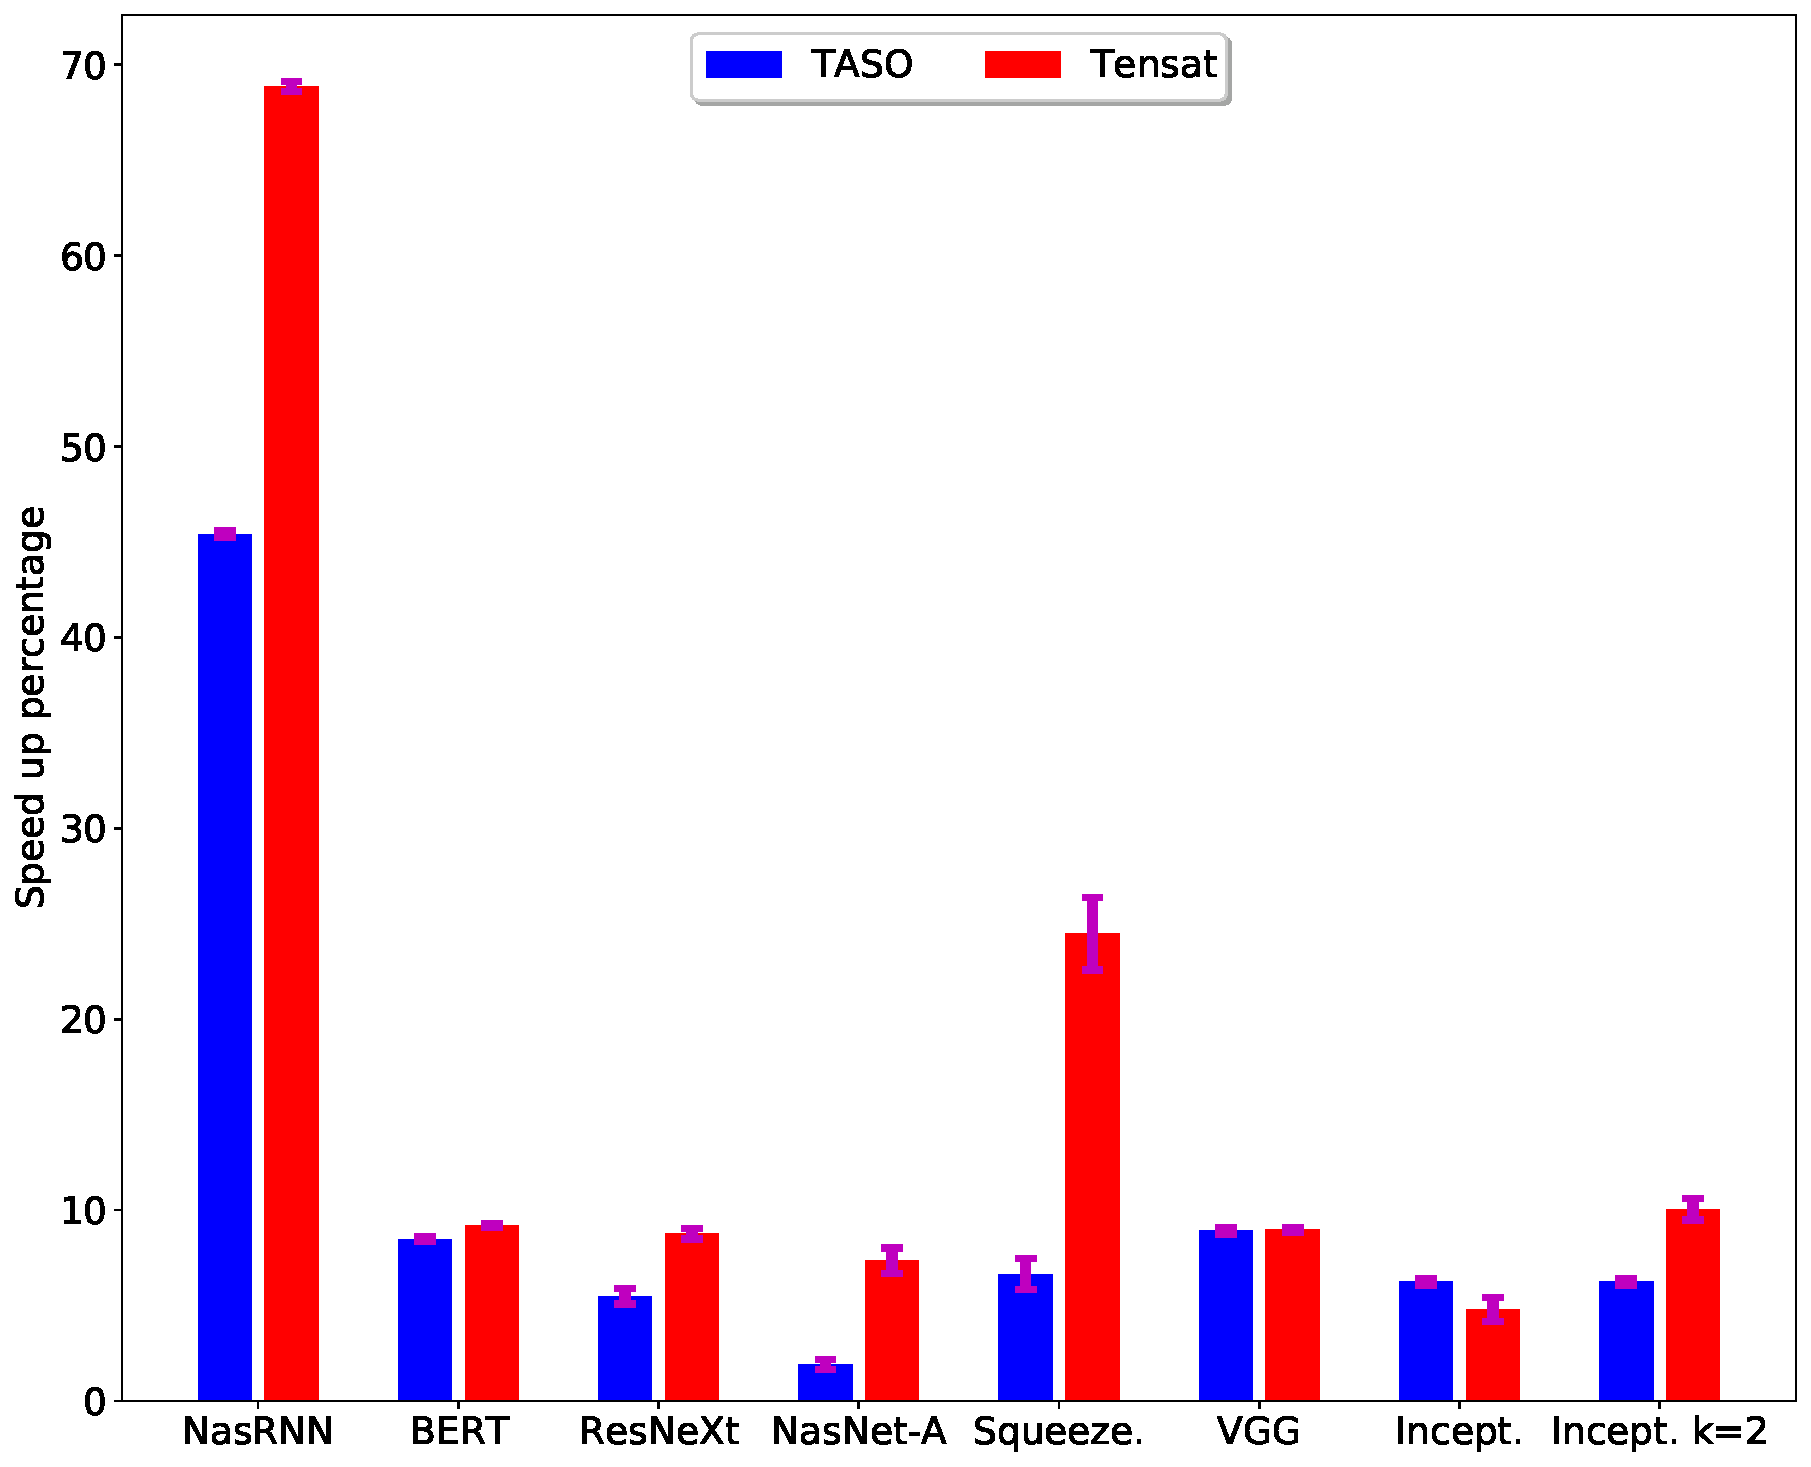
\includegraphics[height=8cm]{tensat/all_speedup.pdf}
  \caption{
    Speedup percentage of the optimized graph with respect to the original graph, TASO v.s. \ourname{}.
    Each setting (optimizer $\times$ benchmark) is run for five times, and we plot the mean and standard error for the measurements.
  }\label{fig:speedup}
  \vspace{2em}

  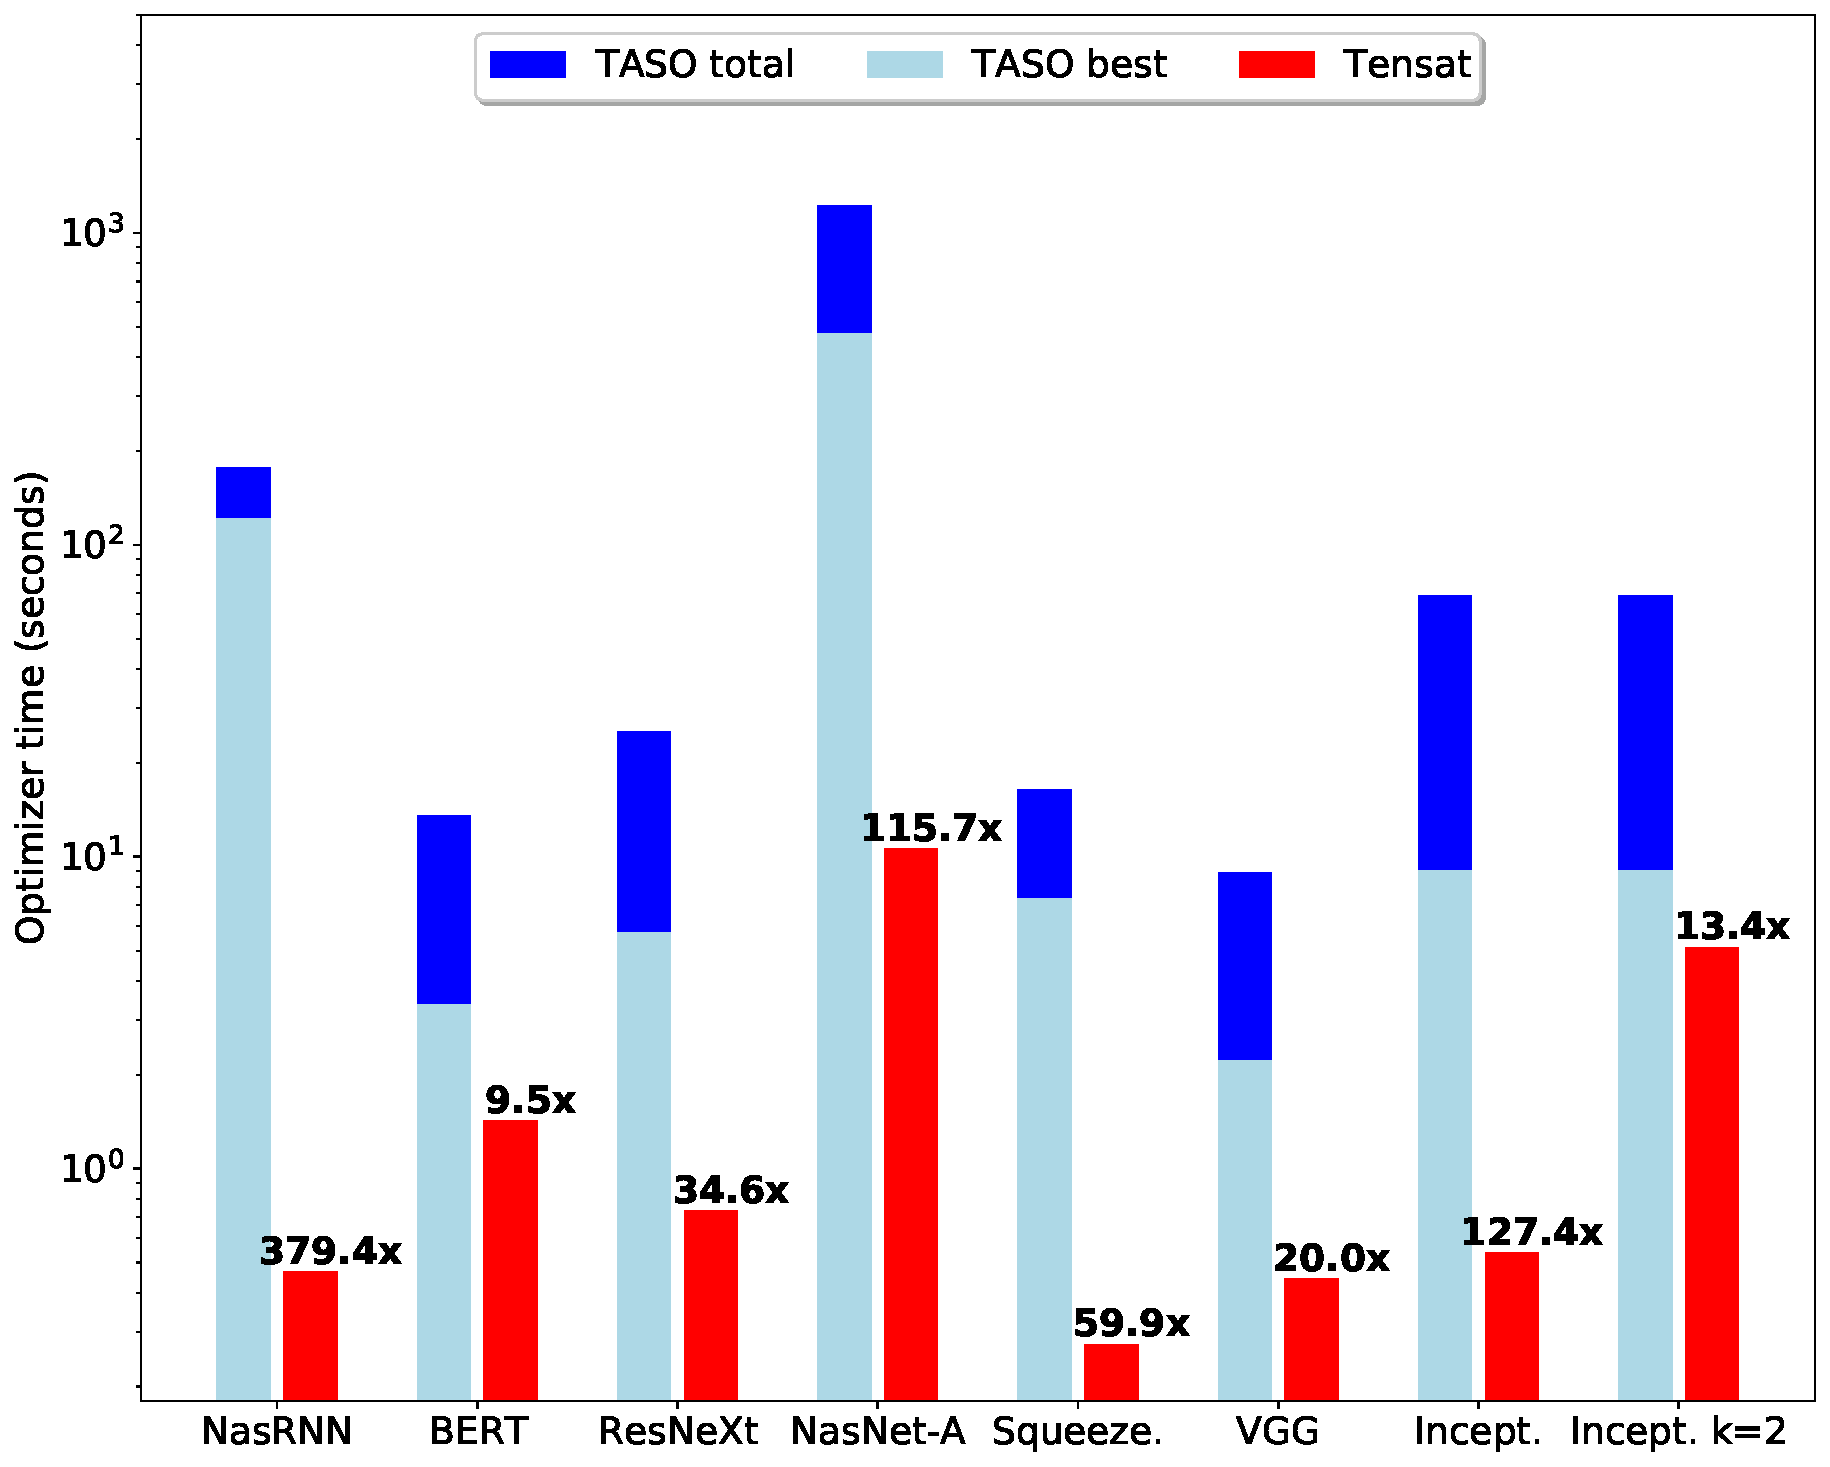
\includegraphics[height=8cm]{tensat/all_optim_time.pdf}
  \caption{
    Comparison of the optimization time (log scale) between TASO and \ourname{}.
    ``TASO total'' is the total time of TASO search.
    ``TASO best'' indicates when TASO found its best result;
    achieving this time would require an oracle telling it when to stop.
  }\label{fig:overhead}
\end{figure}

\paragraph{Program Speedup}
\label{sec:speedup}

We compare the speedup percentage of the optimized graph with respect to the original graph between \ourname{} and TASO.
We use TASO's cuDNN backend to measure the runtime of the full computation graphs.
\autoref{fig:speedup} shows the results.
We can see that \ourname{} discovers better optimized graphs compared with TASO's backtracking search in most benchmarks.
\ourname{}'s optimized graphs are on average 6.6\% faster than TASO's. We see the biggest speedup of 23\% over TASO on NasRNN.
Note that for Inception-v3, \ourname{} with $k_{\textrm{multi}}=1$ gives a smaller speedup than TASO,
but increasing $k_{\textrm{multi}}$ to 2 achieves a better speedup than TASO
while still being 13.4$\times$ faster than TASO's search (see \autoref{fig:overhead}).

This improvement comes from the fact that equality saturation covers a much larger space of equivalent graphs than sequential backtracking search.
By using e-graph as a compact representation of an exponential number of equivalent graphs, \ourname{} is able to cover orders of magnitude more equivalent graphs than TASO.

\paragraph{Optimization Time}
\label{sec:time}

Another important metric is the time taken by the optimizer itself.
For \ourname{}, this is the sum of time taken by the exploration phase and the extraction phase.
For TASO, we record two times for a single backtracking search.
The first is the total time of the backtracking search with the default number of iterations ($T_{\textrm{total}}$).
The second one is the time taken to first reach the best graph found during its search ($T_{\textrm{best}}$).
$T_{\textrm{best}}$ is the best possible time for TASO's sequential backtracking search.
In practice, it is difficult (if not impossible) to achieve $T_{\textrm{best}}$ since the sequential search algorithm would have no way to know that it can stop at that point.

\autoref{fig:overhead} shows the time taken by the optimizers across benchmarks.
We can see that \ourname{} runs 9.5x to 379x faster than TASO's $T_{\textrm{total}}$, and 1.8x to 260x times faster than $T_{\textrm{best}}$.
This shows that \ourname{} can not only cover a much larger search space, but also achieve this in drastically less time.
Furthermore, \ourname{}'s optimization time is small enough that we believe our approach can be integrated into a default compilation flow instead of running the search as an additional offline autotuning process.


% \paragraph{Varying Number of Iterations for Multi-Pattern Rewrites}
% \label{sec:multi-vary}

% As we discuss in \autoref{sec:saturation}, multi-pattern rewrite rules can grow the e-graph in a extremely rapid manner.
% Here we study the effect of varying the number of iterations for multi-pattern rewrites $k_{\textrm{multi}}$.
% \autoref{fig:trend} shows the results.
% We can see the explosion of the number of nodes in the e-graph as $k_{\textrm{multi}}$ increases (due to the double exponential growth).
% For NasRNN, Inception-v3, BERT, NasNet-A, and ResNeXt-50, by increasing $k_{\textrm{multi}}$, \ourname{} discovers better graphs with larger speedups.
% But for SqueezeNet, speedup decreases with $k_{\textrm{multi}}$.
% This is due to the discrepancy between the cost model and the real graph runtime.
% As $k_{\textrm{multi}}$ increases for SqueezeNet, the cost model suggests that certain new rewrites can reduce the cost, while they in fact increase full graph runtime.
% Despite this special case where the discrepancy has an effect, \ourname{} on SqueezeNet with $k_{\textrm{multi}}=3$ still achieves a better speedup than TASO.
% By increasing $k_{\textrm{multi}}$, \ourname{} can explore a larger search space and find better optimized graphs for most benchmarks, at the cost of longer time taken by the optimizer.

% \begin{figure}
%     \centering
%     \includegraphics[width=0.29\hsize]{figures/speedup_trend.pdf}
%     \includegraphics[width=0.29\hsize]{figures/optim_trend.pdf}
%     \includegraphics[width=0.29\hsize]{figures/nodes_trend.pdf}
%     \includegraphics[width=0.09\hsize]{figures/legend_trend.pdf}
%     \caption{Effect of varying the number of iterations of multi-pattern rewrites $k_{\textrm{multi}}$.
%     For BERT, NasNet-A, NasRNN, Inception-v3, the ILP solver times out at one hour for $k_{\textrm{multi}}=3$.
%     Left: speedup of the optimized graphs (the $y$-axis is split for clarity).
%     Middle: time taken by the \ourname{}.
%     Right: final e-graph size (number of e-nodes).
%     The middle and right figures are in log scale.
%     }
%     \label{fig:trend}
% \end{figure}



% \paragraph{Ablation Study}
% \label{sec:ablation}

% In this section, we study the effect of the important design choices in our approach.

% \paragraph{Greedy v.s. ILP extraction}

% The first important design choice is the extraction method.
% \autoref{table:extraction} shows the comparison between greedy extraction and ILP extraction.
% Although greedy extraction works fine on some benchmarks (e.g. NasRNN), it fails to extract an optimized graph on others (e.g. BERT and NasNet-A).
% This is due to the nature of greedy extraction: it makes the choices on which node to pick separately and greedily, without considering the inter-dependencies between the choices.
% Consider the rewrite in \autoref{fig:rewrite} (merging two \texttt{matmul}s by \texttt{concat} and \texttt{split}) as an illustrative example.
% After applying this rewrite to the e-graph, there will be two e-classes that have multiple e-nodes: one e-class per each output.
% This rewrite can reduce the cost only if both e-classes choose the split node, since the RHS subgraph can be reused by the two outputs.
% However, greedy extraction will never pick the split nodes, since it does not know the RHS subgraph is shared between the two split nodes.

% \begin{table}[]
%     \centering
%     \begin{tabular}{cccc}
%     \hline
%         {\bf Graph Runtime (ms)} & {\bf Original} & {\bf Greedy} & {\bf ILP} \\
%     \hline
%         BERT & 1.88 & 1.88 & \textbf{1.73} \\
%         NasRNN & 1.85 & 1.15 & \textbf{1.10} \\
%         NasNet-A & 17.8 & 22.5 & \textbf{16.6} \\
%     \hline
%     \end{tabular}
%     \caption{Comparison between greedy extraction and ILP extraction, on BERT, NasRNN, and NasNet-A.
%     This table shows the runtime of the original graphs and the optimized graphs by greedy extraction and ILP extraction.
%     The exploration phase is run with $k_{\textrm{multi}} = 1$. }
%     \label{table:extraction}
% \end{table}

% \paragraph{ILP with or without cycle constraints}

% Here we study the effect of whether or not to include the cycle constraints in ILP.
% \autoref{table:cycle} presents the effect on extraction time as $k_{\textrm{multi}}$ (thus e-graph size) varies.
% With the cycle constraints, ILP solver time quickly increases with the e-graph size, and reaches timeout when $k_{\textrm{multi}}=2$.
% In our experiments, the ILP solver has not yet found a feasible solution at timeout.
% Removing the cycle constraints leads to approximately 10x--1000x speedup on ILP solving time on larger e-graphs.
% These results show that the main difficulty for the ILP solver is to satisfy the cycle constraints.
% Thus, removing the cycle constraints makes it possible for our approach to scale to larger e-graphs.

% \begin{table}[]
%     \centering
%     \begin{tabular}{ccccc}
%     \hline
%         {\bf Extraction} & \multirow{2}{*}{\bf $k_{\textrm{multi}}$} & \multicolumn{2}{c}{\bf With cycle} & {\bf Without} \\
%         {\bf time (s)} & & real & int & {\bf cycle} \\
%     \hline
%        \multirow{2}{*}{BERT} & 1 & 0.96 & 0.98 & \textbf{0.16} \\
%        & 2 & $>$3600 & $>$3600 & \textbf{510.3} \\
%        \hline
%        \multirow{2}{*}{NasRNN} & 1 & 1116 & 1137 & \textbf{0.32}  \\
%        & 2 & $>$3600 & $>$3600 & \textbf{356.7}  \\
%        \hline
%        \multirow{2}{*}{NasNet-A} & 1 & 424 & 438 & \textbf{1.81}  \\
%        & 2 & $>$3600 & $>$3600 & \textbf{75.1}  \\
%     \hline
%     \end{tabular}
%     \caption{Effect of whether or not to include cycle constraints in ILP on extraction time (in seconds), on BERT, NasRNN, and NasNet-A.
%     For the cycle constraints, we compare both using real variables and using integer variables for the topological order variables $t_m$. }
%     \label{table:cycle}
% \end{table}

% \paragraph{Efficient cycle filtering}

% To remove the cycle constraints from ILP, we need to perform cycle filtering during the exploration phase.
% Here we compare the two cycle filtering techniques introduced in \autoref{sec:cycle}.
% \autoref{table:efficient} shows the effect on the exploration phase time, as $k_{\textrm{multi}}$ varies.
% We can see that the efficient cycle filtering algorithm achieves up to 2000x speedup compared with the vanilla algorithm, making it possible to explore a larger e-graph.

% \begin{table}[]
%     \centering
%     \begin{tabular}{ccccccc}
%     \hline
%         \multirow{2}{*}{$k_{\textrm{multi}}$} & \multicolumn{2}{c}{BERT} & \multicolumn{2}{c}{NasRNN} & \multicolumn{2}{c}{NasNet-A} \\
%         & Van. & Eff. & Van. & Eff. & Van. & Eff. \\
%     \hline
%         1 & 0.18 & \textbf{0.17} & 1.30 & \textbf{0.08} & 3.76 & \textbf{1.27} \\
%         2 & 32.9 & \textbf{0.89} & 2932 & \textbf{1.47} & $>$3600 & \textbf{8.62} \\
%     \hline
%     \end{tabular}
%     \caption{Comparison between vanilla cycle filtering and efficient cycle filtering, on the exploration phase time (in seconds) for BERT, NasRNN, and NasNet-A.}
%     \label{table:efficient}
% \end{table}


%%% Local Variables:
%%% TeX-master: "../thesis"
%%% End: